\section{Resultados}

\subsection{Calibração da XRF}

\begin{frame}
  \frametitle{Calibração da XRF}
  \begin{figure}
      \centering
      \includegraphics[width=0.5\linewidth]{../../outputs/CalibrationK2010MaiAkerr.pdf}
      \includegraphics[width=0.5\linewidth]{../../outputs/CalibrationL2010MaiAkerr.pdf}
  \end{figure}
\end{frame}

\begin{frame}
  \frametitle{Perda de eficiência XRF}
  Comparação das calibrações da XRF-ED nos 3 períodos.
  \begin{figure}[H]
    \begin{subfigure}[b]{0.5\textwidth}
      \includegraphics[width=\textwidth]{../../outputs/CalibrationKcomparacao.pdf}
      \caption{linha K}
    \end{subfigure}%
    \begin{subfigure}[b]{0.5\textwidth}
      \includegraphics[width=\textwidth]{../../outputs/CalibrationLcomparacao.pdf}
      \caption{linha L}
    \end{subfigure}
  \end{figure}
\end{frame}


\begin{frame}
  \frametitle{Comparação das análises de XRF no LAPAt e na US-EPA.}
  \begin{figure}[H]
    \centering
      \includegraphics[width=0.3\textwidth]{../../outputs/epa_iag_S.pdf}
      \includegraphics[width=0.3\textwidth]{../../outputs/epa_iag_K.pdf}
      \includegraphics[width=0.3\textwidth]{../../outputs/epa_iag_Ca.pdf}
  \end{figure}
    \begin{figure}[H]
    	\centering
    	\includegraphics[width=0.3\textwidth]{../../outputs/epa_iag_P.pdf}
    	\includegraphics[width=0.3\textwidth]{../../outputs/epa_iag_Cl.pdf}
    	\includegraphics[width=0.3\textwidth]{../../outputs/epa_iag_V.pdf}
    \end{figure}
\end{frame}

\subsection{Black Carbon}
\begin{frame}
  \frametitle{Calibração do refletômetro usando alvos padrões M71}
  \begin{figure}[H]
    \centering
    \includegraphics[width=0.7\textwidth]{../../outputs/BC_monarch71.pdf}
  \end{figure}
\end{frame}

\begin{frame}
  \frametitle{Padrões produzidos na CETESB com BC ASTM-N762}
  \begin{figure}[H]
  	\centering
  	\includegraphics[width=0.7\linewidth]{../../outputs/BC_cetesb.pdf}
  \end{figure}
\end{frame}

\begin{frame}
  \frametitle{Intercalibração TOT para túnel Jânio Quadros (JQ)}
  \begin{figure}[H]
    \centering
    \includegraphics[width=0.7\linewidth]{../../outputs/JQ_TOT_Refletancia.pdf}
  \end{figure}
\end{frame}

\begin{frame}
  \frametitle{Massa de BC no JQ via intercalibração TOT e padrões CETESB}
  \begin{figure}[H]
    \centering
      \includegraphics[width=0.6\linewidth]{../../outputs/BC_janio_quadros.pdf}
  \end{figure}
\end{frame}

\begin{frame}
  \frametitle{Intercalibração TOT para Acra}
  \begin{figure}[H]
  	\begin{center}
  		\includegraphics[width=0.7\textwidth]{../../outputs/Gana_TOT_Refletancia.pdf}
  	\end{center}
  \end{figure}
\end{frame}

\begin{frame}
  \frametitle{Razão dos valores de BC pelas diferentes calibrações}
  \begin{figure}[H]
  	\centering
  	\begin{subfigure}[b]{0.44\linewidth}
  		\includegraphics[width=\linewidth]{../../outputs/BC_compara_calibs.pdf}
  		\caption{Acra}
  	\end{subfigure}
  		\hspace{0.3cm}
  	\begin{subfigure}[b]{0.44\linewidth}
  		\includegraphics[width=\linewidth]{../../outputs/BC_compara_calibs_recife.pdf}
  		\caption{Recife}
  	\end{subfigure}%
   \end{figure}
\end{frame}

\subsection{Meteorologia}
\begin{frame}
	\frametitle{}
	\begin{figure}[H]
	\centering
		\includegraphics[width=0.8\linewidth]{../../outputs/windRose_mensal.pdf}
    \end{figure}
\end{frame}

\begin{frame}
	\frametitle{}
	\begin{figure}[H]
		\centering
		\includegraphics[width=0.8\linewidth]{../../outputs/windRose_horaria.pdf}
	\end{figure}
\end{frame}


\begin{frame}
\frametitle{}
Intensidade e direção do vento médio na altitude de 
10 e 1000 metros sobre o continente africano.
\begin{figure}[H]
\centering
  \begin{subfigure}[b]{0.5\linewidth}
    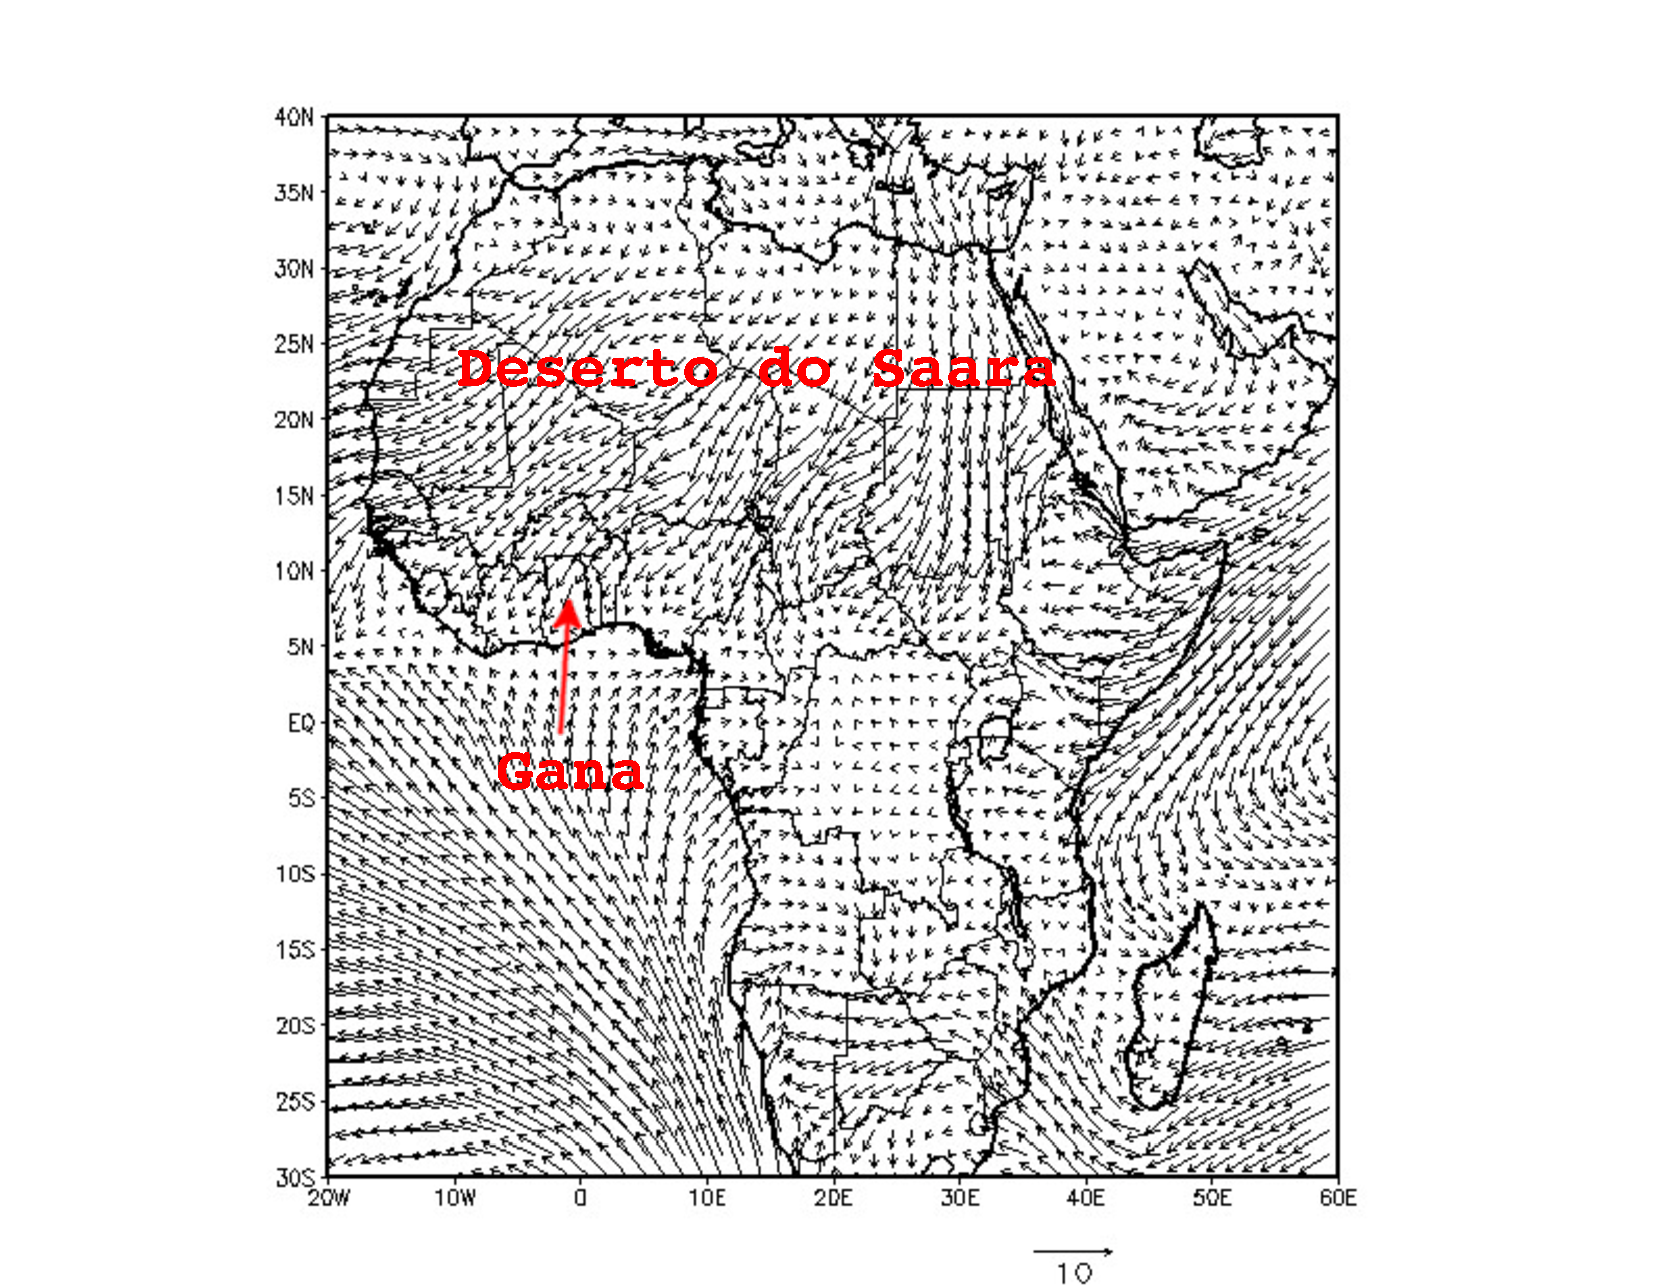
\includegraphics[width=\linewidth]{../../inputs/grads/gimp/1000hPa/JAN_2008.pdf}
    \caption{10 metros}
  \end{subfigure}%
  %  \hspace{0.5cm}
  \begin{subfigure}[b]{0.5\linewidth}
    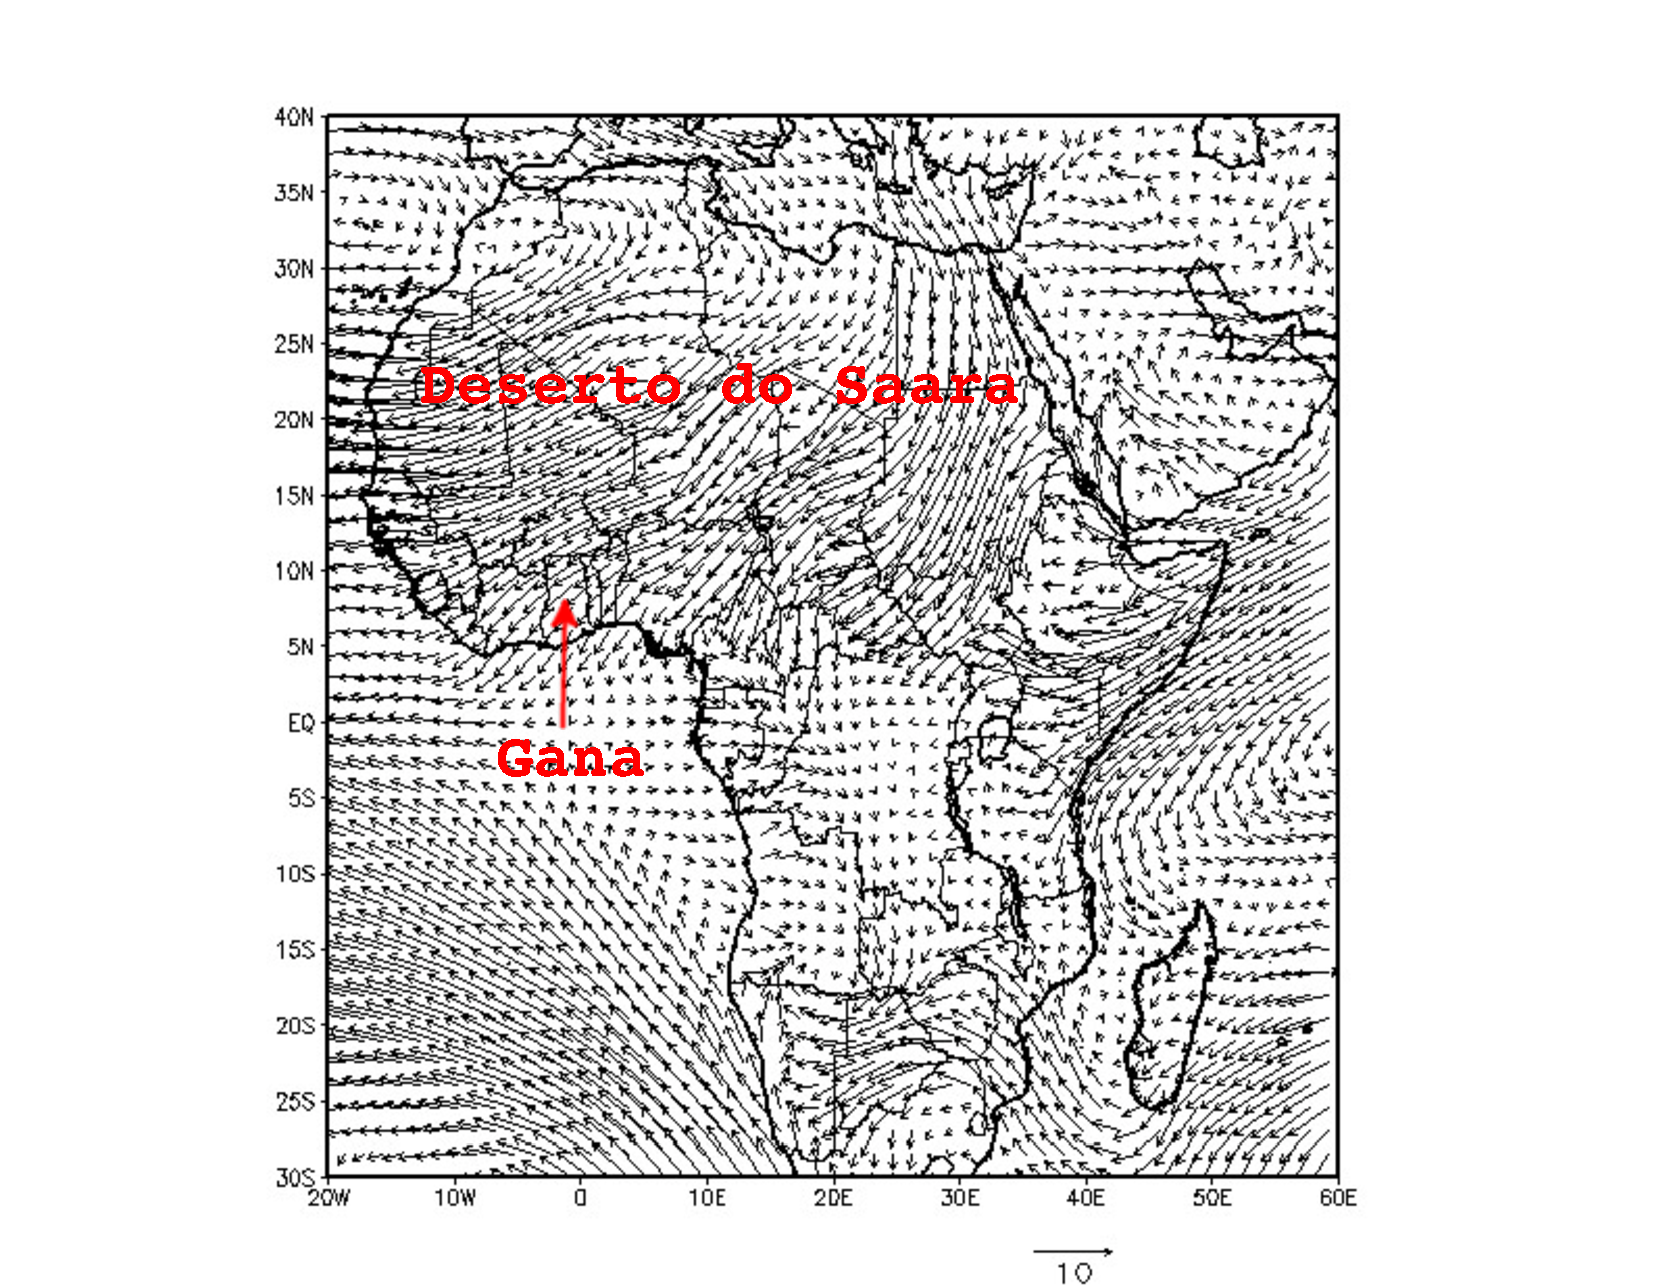
\includegraphics[width=\linewidth]{../../inputs/grads/gimp/875hPa/JAN_2008.pdf}
    \caption{1000 metros}
  \end{subfigure}
\end{figure}
\end{frame}

\subsection{Concentrações Ambientais}
\begin{frame}
  \frametitle{Concentrações Ambientais}
  No Brasil, o padrão anual de $MP_{10}$ é 50 $\mu g/m^3$ e na OMS 20 $\mu g/m^3$. Em Gana, segue legislação vigente:
  \begin{table}[H]
  \centering
  \tiny 
    % http://www.epa.gov.gh/ghanalex/policies/EPAguidelines%20Report.pdf
\begin{tabular}{cccc}
\hline
                              &   regiões  &        zonas       &         zonas               \\
                              & sensíveis  & residenciais e rurais & insdustriais e comerciais      \\
Tipo da média                 & $\mu / m^3$ & $\mu / m^3$ & $\mu / m^3$      \\
\hline
diária                    & 110             & 150                      & 260         \\       
anual geométrica          & 70              & 100                      & 200                   \\
mensal (durante Harmatão) & 100             & 200                      & 500                     \\
\hline
\end{tabular}

  \end{table}
%  \begin{table}[H]
%  \centering
%  \tiny 
%    \begin{tabular}{cccc}
\hline
              & Brasil & Gana (residencial e rural) & OMS \\
Tipo da média & $\mu / m^3$ & $\mu / m^3$ & $\mu / m^3$          \\
\hline
diária   & 150              & 150              &  50             \\
anual    &  50 (aritmética) & 100 (geométrica) &  20 (aritmética) \\
\hline
\end{tabular}

%  \end{table}
Médias de $MP_{10}$ para o ano de 2007:
  \begin{table}[H]
    \centering
    \tiny 
    % latex table generated in R 3.2.4 by xtable 1.7-1 package
% Mon May 16 17:18:28 2016
\begin{tabular}{cccccc|ccccc}
  \hline
  &  \multicolumn{5}{c|}{com Harmatão} & \multicolumn{5}{c}{sem Harmatão} \\
 & n & $\overline{x}^*$ & $\overline{x}_g^{**}$ & $\sigma^{***}$ & $\overline{\sigma}^{***}$
 & n & $\overline{x}^*$ & $\overline{x}_g^{**}$ & $\sigma^{***}$ & $\overline{\sigma}^{***}$ \\
                       \hline & \multicolumn{10}{c}{$\mu g \cdot m^{-3}$} \\  \hline
residencial & 87 & 44,91 & 43,14 & 11,87 & 1,12 & 136 & 115,12 & 67,72 & 186,39 & 13,28 \\ 
  avenida & 89 & 61,57 & 60,55 & 11,52 & 1,08 & 138 & 131,65 & 88,99 & 183,62 & 13,02 \\ 
  ambas & 176 & 53,33 & 51,21 & 14,34 & 0,95 & 274 & 123,45 & 77,70 & 184,85 & 9,29 \\ 
   \hline
\multicolumn{11}{l}{$^{*}$ Média Aritimética} \\
\multicolumn{11}{l}{$^{**}$ Média Geométrica} \\
\multicolumn{11}{l}{$^{***}$ Desvio Padrão} \\
\multicolumn{11}{l}{$^{****}$ Desvio Padrão da Média} \\
   \hline
\end{tabular}

  \end{table}
\end{frame}

\begin{frame}
  \frametitle{Padrão Diário}
    No Brasil, o padrão diário é
    150 $\mu g/m^3$ e na OMS 50 $\mu g/m^3$.
  \begin{figure}[H]
    \centering
    \begin{subfigure}[b]{0.45\textwidth}
      \includegraphics[width=\textwidth]{../../outputs/massa_temporal_RIcH.pdf}
      \caption{Área residencial (Sam Road)}
    \end{subfigure}%
    \begin{subfigure}[b]{0.45\textwidth}
      \includegraphics[width=\textwidth]{../../outputs/massa_temporal_TIcH.pdf}
      \caption{Avenida (Nima Road)}
    \end{subfigure}
  \end{figure}
\end{frame}

\subsection{Identificaçao das fontes}
\begin{frame}
  \frametitle{Identificaçao das fontes}
  
\begin{tcolorbox}[colback=blue!5,colframe=blue!40!black,title=Harmatão]
  Critério para identificação dos dias de ocorrência do Harmatão:
  concentrações de silício no $MP_{10}$ maiores que 10 $\mu g/m^3$ nos  meses de novembro à março. 
\end{tcolorbox}
\end{frame}

\begin{frame}
  \frametitle{Análise de Fatores - Residencial $MP_{2,5}$}        
  \begin{table}[H]
    \centering
    \tiny
    \input{../../outputs/beautifulFAdisplay_RFsH5.tex}
  \end{table}
\end{frame}

\begin{frame}
  \frametitle{Análise de Fatores - Avenida $MP_{2,5}$}    
  \begin{table}[H]
    \centering
    \tiny
    \input{../../outputs/beautifulFAdisplay_TFsH5.tex}
  \end{table}
\end{frame}

\begin{frame}
  \frametitle{PMF - Residencial $MP_{2,5}$}
  Perfil dos fatores em \% e contribuição na massa:
    \begin{figure}
      \centering
            \begin{minipage}[b]{0.4\linewidth}
              \tiny
              \input{../../outputs/RFsH_profiles_percent_species5.tex}
            \end{minipage}
                  \hspace{3cm}
      \begin{minipage}[b]{0.3\linewidth}
        \includegraphics[width=\linewidth]{../../outputs/RFsH_pmf_contribution_pizza5.pdf}

      \end{minipage}%\hfill
    \end{figure}
\end{frame}

\begin{frame}
  \frametitle{PMF - Avenida $MP_{2,5}$}
  Perfil dos fatores em \% e contribuição na massa:
    \begin{figure}
      \centering
            \begin{minipage}[b]{0.4\linewidth}
              \tiny
              \input{../../outputs/TFsH_profiles_percent_species5.tex}
            \end{minipage}
                  \hspace{3cm}
      \begin{minipage}[b]{0.3\linewidth}
        \includegraphics[width=\linewidth]{../../outputs/TFsH_pmf_contribution_pizza5.pdf}
      \end{minipage}%\hfill
    \end{figure}
\end{frame}

\begin{frame}
  \frametitle{Síntese dos fatores extraídos para $MP_{2,5}$}
  \begin{table}[H]
    \centering
    \tiny
    \begin{tabular}{llll|lll}
\hline
                                                  &                        & \multicolumn{5}{c}{Residencial (massa média 27,52 $\mu g / m^3$)}     \\
                                                  &                        & \multicolumn{2}{c}{AF}      & \multicolumn{3}{c}{PMF}                   \\
\hline
 & & & & \multicolumn{3}{c}{contribuição na massa}  \\
Fonte associada                                   & Elementos majoritários & $NF^1$   & VE$^2$ (\%)               & $NF^1$   & (\%)   & $\mu g / m^3$  \\
\hline
\textbf{Solo}                                     & Mg,Al,Si,Ca,Ti,V,Mn,Fe & 1   & 43,78                 & 3   & 22,2         & \textbf{6,11}   \\
\textbf{Queima biomassa}                          & P,S,K,BC                  & 2   & 12,36                 & 5   & 21,6         & \textbf{5,94}  \\
\textbf{Veículos}                                 & BC,Zn,K,Pb             & 3   & 11,24                 & 1   & 40,0           & \textbf{11,01}   \\
\textbf{Mar}                                      & Na,Cl                  & 4   & 8,81                  & 4   & 11,6         & \textbf{3,19}    \\
\textbf{Queima lixo} & Br,Pb                      & 5   & 7,40                   & 2   & 4,65         & \textbf{1,28}   \\

\hline
\multicolumn{7}{l}{$^1$ NF: Número do Fator} \\
\multicolumn{7}{l}{$^2$ VE: Variância Explicada} \\
\hline
\end{tabular}


  \end{table}
  
    \begin{table}[H]
    	\centering
    	\tiny
    	\begin{tabular}{llll|lll}
\hline
                                                  &                        & \multicolumn{5}{c}{Avenida (massa média 31,9 $\mu g / m^3$)}    \\
                                                  &                        &  \multicolumn{2}{c}{AF}                      & \multicolumn{3}{c}{PMF}          \\
\hline
 & & & & \multicolumn{3}{c}{contribuição na massa} \\
Fonte associada                                   & Elementos majoritários & $NF^1$       & VE$^2$  (\%)            & $NF^1$ & (\%)  & $\mu g / m^3$ \\
\hline
\textbf{Solo}                                     & Mg,Al,Si,Ca,Ti,V,Mn,Fe & 1       & 45,49               & 3 & 22,2        & \textbf{7,08}  \\
\textbf{Queima biomassa}                          & P,S,K,BC                  &  2       & 13,44               & 4 & 28,8        & \textbf{9,19}  \\
\textbf{Veículos}                                 & BC,Zn,K,Pb             &  5       & 7,19                & 5 & 31,5        & \textbf{10,05} \\
\textbf{Mar}                                      & Na,Cl                  &  3       & 9,76                & 2 & 13,6        & \textbf{4,34}  \\
\textbf{Queima lixo} & Br,Pb                      &  4       & 8,73                & 1 & 3,86        & \textbf{1,23} \\

\hline
\multicolumn{7}{l}{$^1$ NF: Número do Fator} \\
\multicolumn{7}{l}{$^2$ VE: Variância Explicada} \\
\hline
\end{tabular}


    \end{table}
\end{frame}

\begin{frame}
  \frametitle{Análise de Fatores - Residencial $MP_{2,5-10}$}        
  \begin{table}[H]
    \centering
    \tiny
    \input{../../outputs/beautifulFAdisplay_RGsH4.tex}
  \end{table}
\end{frame}

\begin{frame}
  \frametitle{Análise de Fatores - Avenida $MP_{2,5-10}$}    
  \begin{table}[H]
    \centering
    \tiny
    \input{../../outputs/beautifulFAdisplay_TGsH4.tex}
  \end{table}
\end{frame}

\begin{frame}
  \frametitle{PMF - Residencial $MP_{2,5-10}$}
  Perfil dos fatores em \% e contribuição na massa:
    \begin{figure}
      \centering
            \begin{minipage}[b]{0.4\linewidth}
              \tiny
              \input{../../outputs/RGsH_profiles_percent_species4.tex}
            \end{minipage}
                  \hspace{3cm}
      \begin{minipage}[b]{0.3\linewidth}
        \includegraphics[width=\linewidth]{../../outputs/RGsH_pmf_contribution_pizza4.pdf}
      \end{minipage}%\hfill
    \end{figure}
\end{frame}

\begin{frame}
  \frametitle{PMF - Avenida $MP_{2,5}$}
  Perfil dos fatores em \% e contribuição na massa:
    \begin{figure}
      \centering
            \begin{minipage}[b]{0.4\linewidth}
              \tiny
              \input{../../outputs/TGsH_profiles_percent_species4.tex}
            \end{minipage}
                  \hspace{3cm}
      \begin{minipage}[b]{0.3\linewidth}
        \includegraphics[width=\linewidth]{../../outputs/TGsH_pmf_contribution_pizza4.pdf}
      \end{minipage}%\hfill
    \end{figure}
\end{frame}

\begin{frame}
	\frametitle{Síntese dos fatores extraídos para $MP_{2,5-10}$}
	\begin{table}[H]
		\centering
		\tiny
		\begin{tabular}{llll|lll}
\hline
                                                  &                        & \multicolumn{5}{c}{Residencial (massa média 25,26 $\mu g / m^3$)}     \\
                                                  &                        & \multicolumn{2}{c}{AF}      & \multicolumn{3}{c}{PMF} \\
\hline
 & & & & \multicolumn{3}{c}{contribuição na massa} \\
Fonte associada                                   & Elementos majoritários & $NF^1$   & VE$^2$ (\%)               & $NF^1$   & (\%)   & $\mu g / m^3$ \\
\hline
\textbf{Solo}                                                    & Mg, Al, Si, Ca,Ti, V, Mn, Fe & 1  & 49,07               & 1      & 29,18 & \textbf{7,37}  \\
\textbf{Envelhecido} & S, K, Zn, Br, Pb             & 2  & 24,25               & 4      & 22,36 & \textbf{5,65}  \\
\textbf{Mar}                                                     & Na,Cl                        & 3  & 12,34               & 3      & 16,36 & \textbf{4,13}  \\
\textbf{Poeira de estrada}                                       & solo + Zn                       & 4  & 7,69                & 2      & 32,09 & \textbf{8,11} \\ 

\hline
\multicolumn{7}{l}{$^1$ NF: Número do Fator} \\
\multicolumn{7}{l}{$^2$ VE: Variância Explicada} \\
\hline
\end{tabular}

	\end{table}
	
	\begin{table}[H]
		\centering
		\tiny
		\begin{tabular}{llll|lll}
\hline
                                                  &                         & \multicolumn{5}{c}{Avenida (massa média 33,23 $\mu g / m^3$)}    \\
                                                  &                         & \multicolumn{2}{c}{AF}                    & \multicolumn{3}{c}{PMF}          \\
\hline
 &  & & & \multicolumn{3}{c}{contribuição na massa} \\
Fonte associada                                   & Elementos majoritários & $NF^1$       & VE$^2$  (\%)            & $NF^1$ & (\%)  & $\mu g / m^3$ \\
\hline
\textbf{Solo}                                                    & Mg, Al, Si, Ca,Ti, V, Mn, Fe &  1  & 51,46               & 3      & 35,63 & \textbf{11,84} \\
\textbf{Envelhecido} & S, K, Zn, Br, Pb             & 2& 16,57               & 4      & 10,29 & \textbf{3,42}  \\
\textbf{Mar}                                                     & Na,Cl                        &  3  & 13,55               & 1      & 26,53 & \textbf{8,82}  \\
\textbf{Poeira de estrada}                                       & solo + Zn                       &  4  & 6,96                & 2      & 27,56 & \textbf{9,16}   \\ 

\hline
\multicolumn{7}{l}{$^1$ NF: Número do Fator} \\
\multicolumn{7}{l}{$^2$ VE: Variância Explicada} \\
\hline
\end{tabular}

	\end{table}
\end{frame}
